\section{Attitude Determination and Control Subsystem}
\subsection{Selection of Magnetorquers}
The SnapSat is a relatively small satellite with low mass and power considerations.
After extensive literature review it was determined that given the mass and power consideration of the SnapSat, magnetorquers would provide a better controls system than 

\subsection{Design of Magnetorquer}
The torque on the satellite produced by the magnetorquer is given by cross product of the magnetic dipole of the magnetorquer and the earths magnetic field strength: 
\begin{center}
$T = M \times B$
\end{center}
It is impossible to change the earth's magnetic field strength which is approximately $3 \times 10^{-6}$ Tesla.  Thus in order to maximise the torque on the satellite the magnetic dipole must be maximised. The magnetic dipole for the magnetorquer is given by the following equation:
\begin{center}
$M = N \cdot I \cdot A$
\end{center}
Thus the magnetic dipole is dependent on the number of turns in the coil, the current through the wire and the area of the coil.  Initially it seems like a simple problem where the dipole will simply increase with the number of turns if the current and area are held constant.  However, this view does not take into account the resistance that increases with the length of wire, which given the fixed voltage will limit the current.  Due to cost restrictions, only 0.18mm round copper wire was available for use, which had a resistance per metre ($R_m$) of 0.646 ohms.  The following equations were then combined with the magnetic dipole equation in order to optimise the number of turns required:
\begin{center}
$I = \frac{V}{R}$\vspace{2mm}\\
$R = N \cdot Perimeter \cdot R_m$ \vspace{2mm}\\
$P = V \cdot I$
\end{center}
When combined the following equation was determined:
\begin{center}
$1 = \frac{4 \cdot M \cdot R_m}{V \cdot A}$
\end{center}
Thus since resistance per metre and voltage are constant, and perimeter is dependent on area, the magnetic dipole becomes constant for a given area.  Due to the restrictions in the lab only two sizes were available for the magnetorquers. The larger size was selected with side lengths of 0.073m as when the smaller size was modelled, the current draw was too high causing a higher level of power to be used.  Thus given this fixed area, the maximum magnetic dipole was determined to be  0.14$Am^2$.  Using this maximum dipole as the basis, the other characteristics of the magnetorquer were determined and can be viewed in the table below.




\begin{table}[H]
\begin{center}
\caption{Predicted Data for the Magnetorquers}
\begin{tabular}{|c|c|c|c|c|c|c|c|}
\hline
Magnetic Dipole & Number of Turns & Current & Area & Voltage & Resistance & Power Required\\
\hline
0.14$Am^2$ & 132 & 0.2A & 0.005329$m^2$ & 5V & 24.9$\Omega$ & 1W\\
\hline
\end{tabular}
\end{center}
\vspace{-6mm}
\end{table}

\subsection{Construction of Magnetorquers}
As mentioned previously the Magnetorquers were built in house using equipment provided in the space lab.  The following procedure was applied to make each magnetorquer:
\begin{enumerate}
	\item The metal structural mould for the magnetorquer was unscrewed and sticky tape was applied to areas that were likely to come into contact with glue.
	\item The mould was placed in the winder and the copper wire was set up as shown in the photographs below.
	\begin{center}
	\begin{figure}[H]
	\caption{Magnetorquer Construction Set Up}
	\begin{subfigure}{0.5\textwidth}
	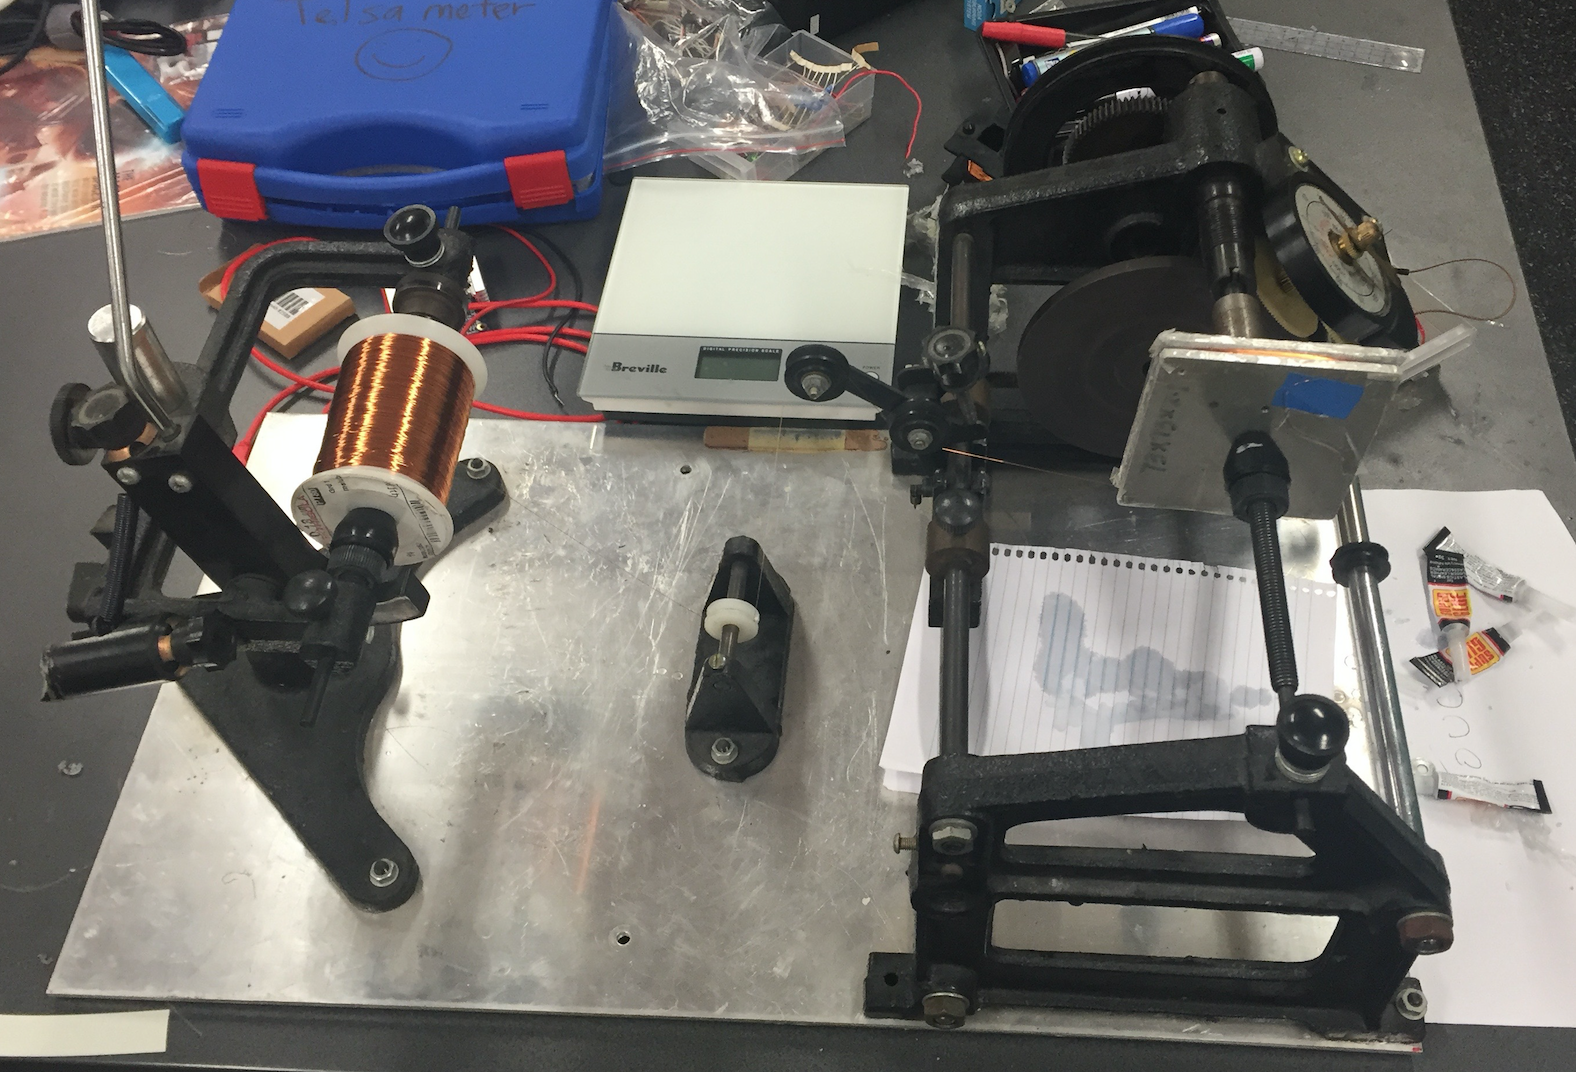
\includegraphics[scale = 0.35]{Construction_1.png}
	\end{subfigure}
	\hspace{10mm}
	\begin{subfigure}{0.5\textwidth}
	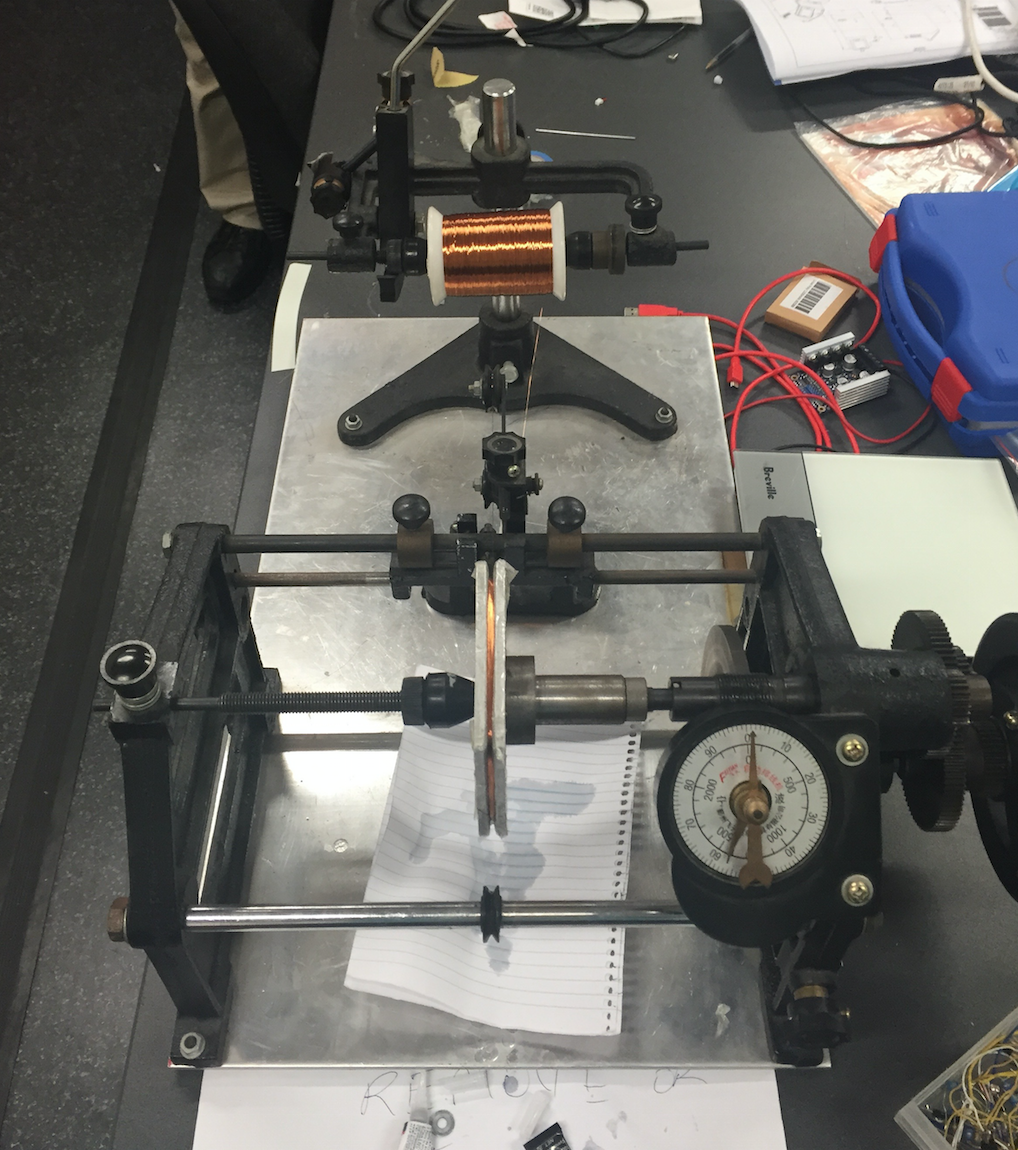
\includegraphics[scale = 0.35]{Construction_2.png}
	\end{subfigure}
	\end{figure}
	\end{center}
	\vspace{-5mm}
	
	
	\item The wire at the very beginning of the coil was taped to the side of the mould to keep it separate from the coil so that it can be connected to the PCB.
	\item In order to measure the number of turns, the counter on the winder was set to zero.
	\item Twenty turns were completed and then a layer of super glue was added to the coiled wire on all four sides in order using a thin brush.
	\item Step 4 was repeated until the required number of turns was reached at which point another layer of glue was added to each side of the coil.
	\item The copper wire was cut and the wire at the very end of the coil was not stuck to the the main coil in order to provide a connection between the PCB and the magnetorquer.
	\item The glue was allowed to set for 10 mins and then the coil was carefully removed from the mould with the aid of the sticky tape.
	\item Once completed the ends of coil were carefully scraped with sandpaper in order to remove the protective coating and allow current to be passed through.
	\item The coil was testing by attaching it to a battery and using a compass to determine whether a magnetic field was being produced.
	\item An Ohmmeter was used to determine the resistance through the coil.  
\end{enumerate}
After testing both magnetorquers were found to have a slightly higher resistance than predicted with the first magnetorquer reading a resistance of 27.2$\Omega$ and the second magnetorquer reading 28.1$\Omega$.  This is roughly a 10\% increase on the predicted value of 24.9$\Omega$ and is most likely caused by the effect of the super glue which was not taken into consideration in the original calculations.  This will result in the magnetorquers using a slightly lower current as voltage is constant and have a lower maximum dipole value.  These values were calculated to be 0.138$Am^2$ and 0.137$Am^2$ for magnetorquers 1 and 2 respectively.  The image below depicts magnetorquer 1 just after construction.

\vspace{-6mm}
\begin{center}
\begin{figure}[H]
\caption{Completed Magnetorquer}
\vspace{-4mm}
\centering
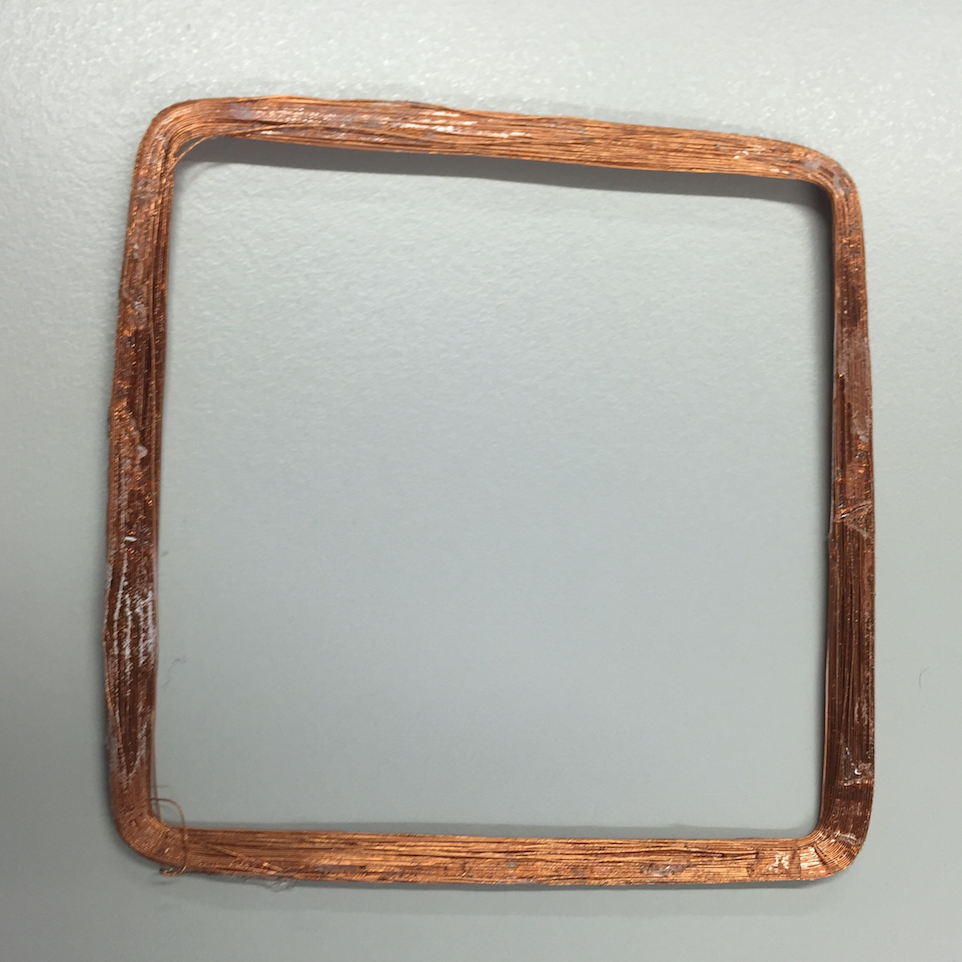
\includegraphics[scale = 0.4]{Magnetorquer.png}
\end{figure}
\end{center}
\vspace{-5mm}

\subsection{Magnetorquer Control System}
The dynamic model for the magnetorquer control system was produced by three fundamental equations:
\begin{center}
$T = N \cdot I \cdot A \cdot B \cdot sin(\theta)$ \vspace{2mm} \\
$V = I \cdot R$\vspace{2mm}\\
$T = J \cdot \ddot{\theta}$\\
\end{center}
By combining these three equations and using a Laplace transform the following dynamic model was determined:
\begin{center}
$\frac{\theta(s)}{V(s)} = \frac{N \cdot A \cdot B}{J \cdot R \cdot s^2 (s^2 + 1)}$
\end{center}
Thus using this function the following Simulink model was produced to determine the expected response of the satellite given certain inputs.

\vspace{-6mm}
\begin{center}
\begin{figure}[H]
\caption{Simulink Model of Control System}
\vspace{-4mm}
\centering
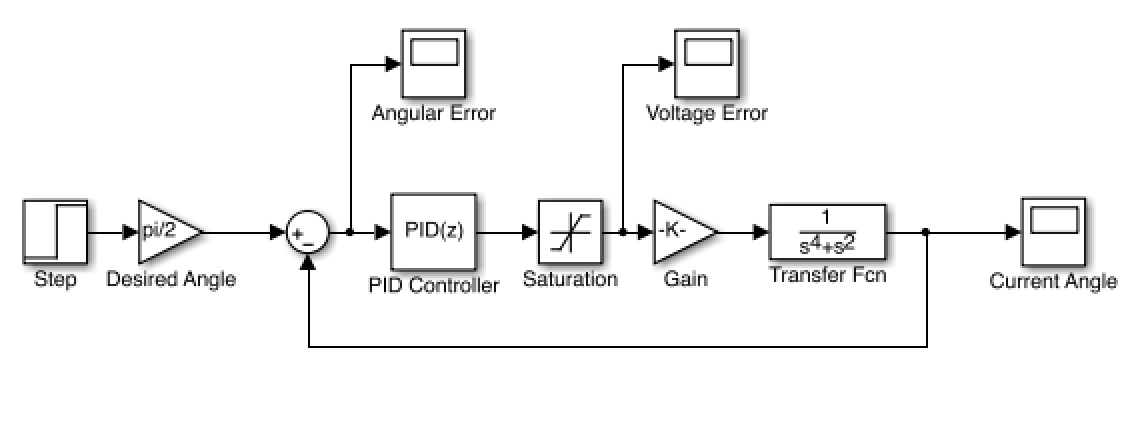
\includegraphics[scale = 0.8]{Simulink_ADCS_Model.png}
\end{figure}
\end{center}
\vspace{-5mm}

